%%%%%%%%%%%%%%%%%%%%%%%%%%%%%%%%%%%%%%%%%%%%%%%%%%%%%%%%%%%%%%%%%%%%%%%%%%%%%%%%
%2345678901234567890123456789012345678901234567890123456789012345678901234567890
%        1         2         3         4         5         6         7         8

\documentclass[letterpaper, 10 pt, conference]{ieeeconf}  % Comment this line out if you need a4paper

%\documentclass[a4paper, 10pt, conference]{ieeeconf}      % Use this line for a4 paper

\IEEEoverridecommandlockouts                              % This command is only needed if 
                                                          % you want to use the \thanks command

\overrideIEEEmargins       
\usepackage{todonotes}                              
\RequirePackage{graphicx}
\graphicspath{ {figures/} }
% See the \addtolength command later in the file to balance the column lengths
% on the last page of the document

% The following packages can be found on http:\\www.ctan.org
%\usepackage{graphics} % for pdf, bitmapped graphics files
%\usepackage{epsfig} % for postscript graphics files
%\usepackage{mathptmx} % assumes new font selection scheme installed
%\usepackage{times} % assumes new font selection scheme installed
%\usepackage{amsmath} % assumes amsmath package installed
%\usepackage{amssymb}  % assumes amsmath package installed

\title{\LARGE \bf
Preparation of Papers for IEEE Sponsored Conferences \& Symposia*
}


\author{Albert Author$^{1}$ and Bernard D. Researcher$^{2}$% <-this % stops a space
\thanks{*This work was not supported by any organization}% <-this % stops a space
\thanks{$^{1}$Albert Author is with Faculty of Electrical Engineering, Mathematics and Computer Science,
        University of Twente, 7500 AE Enschede, The Netherlands
        {\tt\small albert.author@papercept.net}}%
\thanks{$^{2}$Bernard D. Researcheris with the Department of Electrical Engineering, Wright State University,
        Dayton, OH 45435, USA
        {\tt\small b.d.researcher@ieee.org}}%
}


\begin{document}

\maketitle
\thispagestyle{empty}
\pagestyle{empty}


%%%%%%%%%%%%%%%%%%%%%%%%%%%%%%%%%%%%%%%%%%%%%%%%%%%%%%%%%%%%%%%%%%%%%%%%%%%%%%%%
\begin{abstract}
This paper proposes a closed-loop testing setup for pacemakers, in which the pacemaker is connected to a Virtual Heart Model (VHM) and both device and heart signals are used to assess correctness of the device's operation. 
The test inputs are automatically generated by a requirements-guided algorithm that uses the desired heart behavior as a guide for finding test cases that violate it.
These can be replayed by the designer to determine whether the pacemaker operated incorrectly.
The advantages of closed-loop testing over open-loop testing are illustrated with two experiments involving the VHM and a validated pacemaker model.
\end{abstract}
\section{Introduction}
\label{introduction}



%\section{Heart and Pacemaker Basics}
\label{basics}
In this section, we review basic concepts related to the heart and its electrical conduction system which interacts with the pacemaker. 
In-depth material of cardiac electro-physiology can be found in \cite{fogoros}. 

\subsection{Basics of Cardiac Electrophysiology Operation}
The coordinated contraction of the heart is governed by its Electrical Conduction System (see \ref{conduction}). The Sinoatrial (SA) node, which is a collection of specialized tissue at the upper right atrium, spontaneously generates periodical electrical pulses that can cause muscle contraction. 
The SA node acts as the natural pacemaker of the heart. 
The electrical pulses first cause both atria to contract, forcing the blood into the ventricles. 
The electrical conduction is then delayed at the Atrioventricular (AV) node, allowing the ventricles to fill fully. Finally, the fast-conducting His-Pukinje system spreads the electrical activation within both ventricles, causing simultaneous contraction of the ventricular muscles, and pumps the blood out of the heart. 
Appropriate timing is key to proper heart rhythm.

\begin{figure}
  	\begin{center}
    	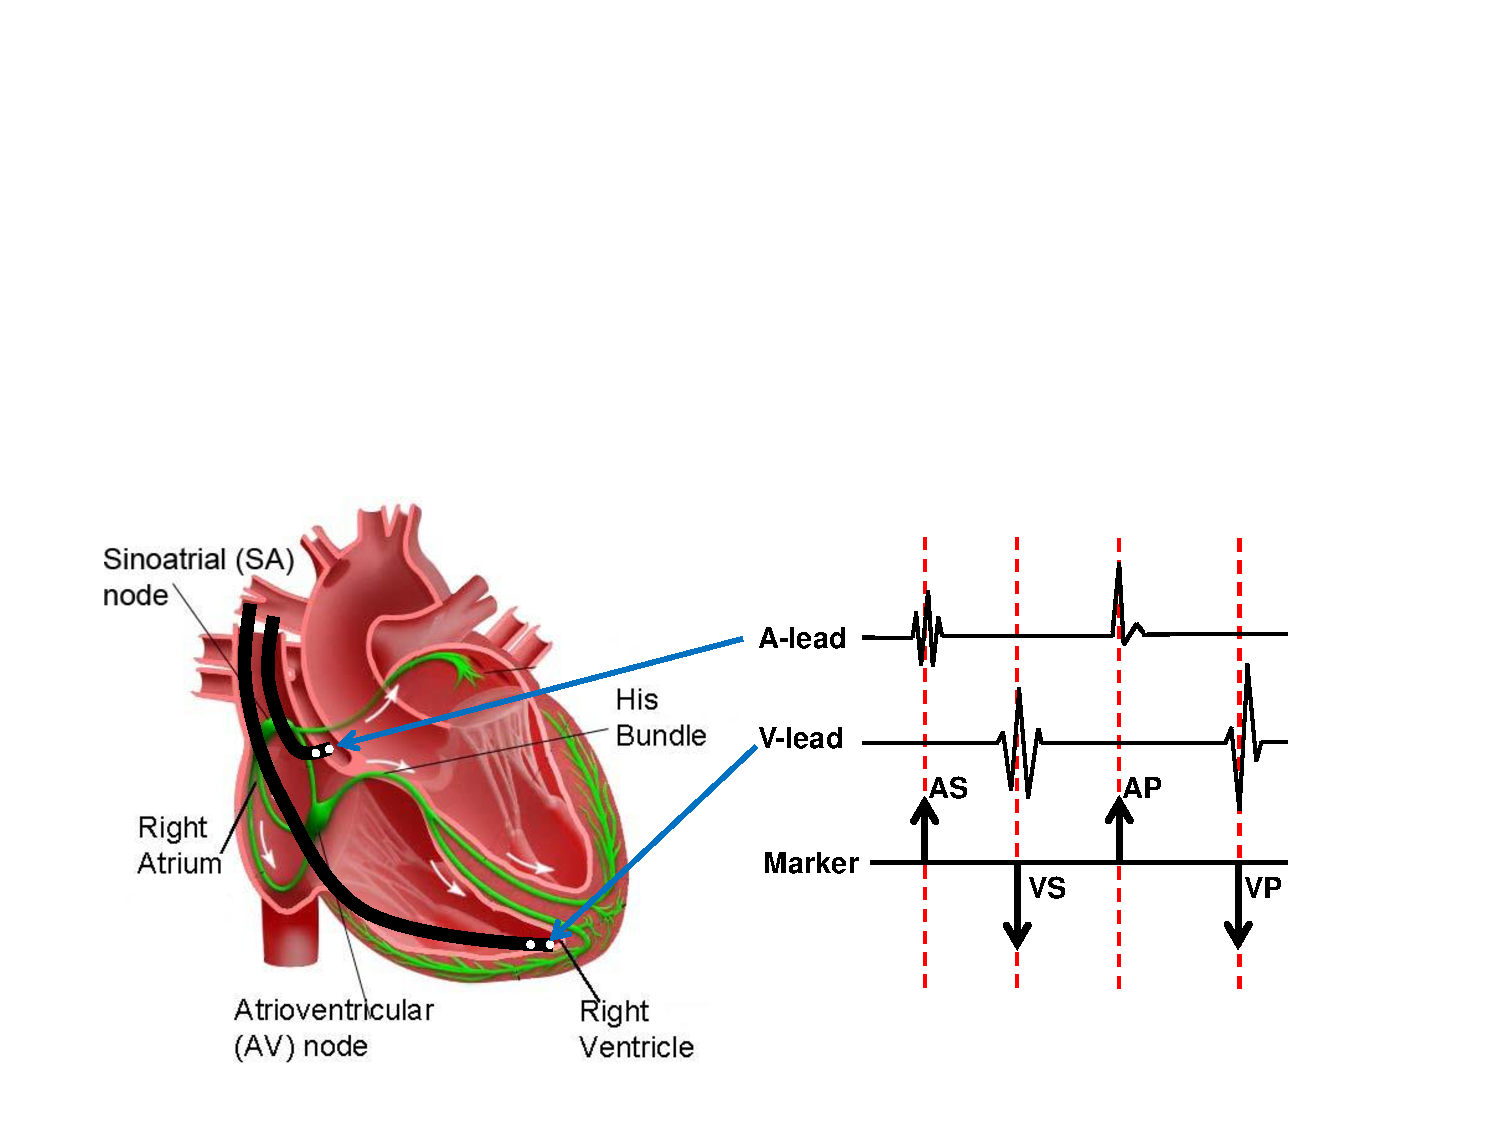
\includegraphics[width=0.45\textwidth]{figures/egm.pdf}
  	\end{center}
	\caption{\small (a) Electrical Conduction System of the Heart and pacemaker leads location. (b) Electrical signal sensed from the pacemaker leads are converted to event markers (AS,VS). Pacemaker delivers electrical pacing (AP,VP) from corresponding leads when heart rate is slow.}
	\label{fig:conduction}
\end{figure}

Due to various factors such as aging and disease, the conduction properties of heart tissue may change. 
These changes often cause timing anomalies in heart rhythm, thus decreasing the blood pumping efficiency of the heart. These timing anomalies are referred to as \emph{arrhythmias}.  

%\subsection{Interfacing the Heart with the Pacemaker}
\label{interfacingHeartPM}



\subsection{Limitations of Current Practice: Open-loop Testing of Pacemakers}
\label{todaysPractice}
\begin{figure}[tb]
	\centering
	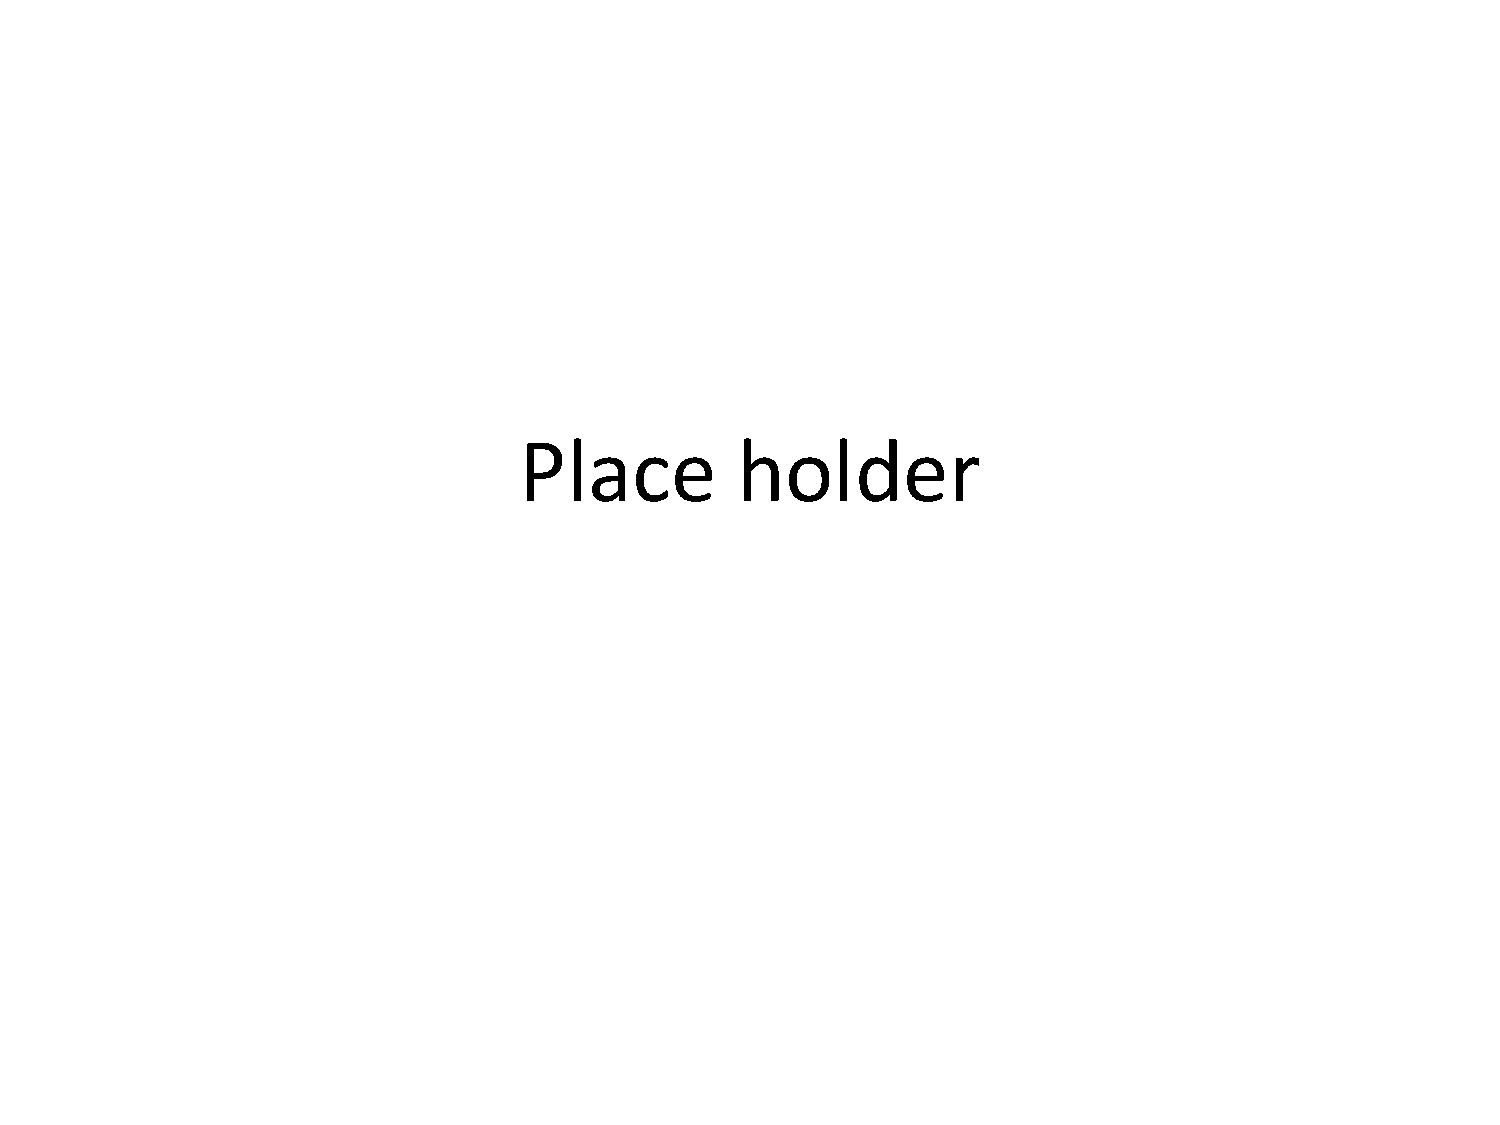
\includegraphics[scale=0.2]{placeHolder.pdf}
	\caption{Setup for pacemaker operation: the device (pacemaker), the plant (human heart), external disturbances (PVCs and PACs), and initial states and parameters (refractory periods, various settings).}
	\label{fig:liveSetup}
\end{figure}
Consider Fig.\ref{fig:liveSetup}, where a typical setup of pacemaker operation is presented.
The Device Under Test (DUT) is connected to the Plant (here, a human heart) which it is meant to control.
Together, they are referred to as the \emph{closed loop}, whereas the DUT alone is an \emph{open loop}.
The plant receives inputs from the DUT, but can also be subject to \emph{external disturbances}: in our case, we consider PVCs and PACs to be external disturbances.
The terminology is meant to convey that these disturbances are inputs to the heart that do not originate in the DUT, but elsewhere. 
The origin of these disturbances need not be modeled.  
They are \emph{disturbances} because they are uncontrolled and can prevent the closed loop from achieving its objectives, namely, a safe and reliable heart operation.

The outputs of the pacemaker are denoted by the letter $u$, e.g. $u = [A_{pace}, V_{pace}]$.
Let $U$ be the set of possible $u$ values.
These constitute inputs to the heart, or plant.
The outputs of the heart are denoted by the letter $y$, e.g. $y = [A_{sense}, V_{sense}]$.
Let $Y$ be the set of possible $y$ values.
These constitute inputs to the pacemaker, or DUT.
A finite sequence, or \emph{string}, of $u$ values will be denoted by $\ub$, and the set of \emph{all} finite $u$-sequences will be denoted by $U^*$: $\ub \in U^*$.
Similarly, we define $\yb \in Y^*$ to be a finite $y$-string.
The disturbances are denoted by $w$, their set of possible values by $W$, and strings of disturbance values by $\wb \in W^*$.

A (discrete-time) \emph{open-loop test} $\yb$ for the DUT is a string $\yb = y_1 y_2 \ldots y_n \in Y^*$.
As a result of being fed a test, the DUT will synchronously produce a string $\ub = u_1 \ldots u_n \in U^*$.
A (discrete-time) \emph{closed-loop test} $\wb$ for the closed loop DUT+Plant (pacemaker + heart) is a string $\wb = w_1 w_2 \ldots w_n \in W^*$.
As a result of being fed a test, the closed loop will synchronously produce a string $(\ub,\yb) \in U^* \times Y^*$.
%The plant $\Hc$ may be seen as an input-output map: $\Hc: U^* \rightarrow Y^*$, where $U^* (Y^*)$ is the set of finite strings over the set $U$ ($Y$).

\subsection{Testing objectives}
\label{testingObjectives}
When testing a pacemaker, or any device in general, two crucial decisions must be made:
\begin{itemize}
	\item Choice of inputs: first, what input strings should be provided to the device so its behavior can be observed in reaction to them? 
	Ideally, the answer is: all input sequences that might be produced by the heart to which the device will be connected. 
	Sequences from outside this set are irrelevant, and missing sequences from within this set might cause us to miss some bugs that will manifest themselves during live operation.
	In what follows, we use $A_\Hc$ to denote the set of strings that might be produced by the heart when connected to the pacemaker in a closed loop as shown in Fig.\ref{fig:liveSetup}. 
	Of course, $A_\Hc \subset Y^*$.
	\item Criterion of correctness: secondly, how do we determine that a particular operation of the device is correct? 
	In other words, what is the specification according to which the device is being tested?
	Ideally, the answer is: the specification will describe the safe, acceptable operation of the heart. 
	I.e. the device is correct if the heart it is controlling does not produce unsafe or undesirable behavior.
	Because the heart is a complex system and its `acceptable' behavior is dependent on its structural characteristics and current condition, such specifications are hard to describe. 
	Nonetheless, this is the standard for what a specification should be for the DUT. 
	A DUT that violates this specification may or may not be modified, depending on the source of the violation. 
	The task of interpreting test outcomes and acting upon them is left to the designer and physician.	
	The validation engineer's task is to produce a trace that violates the specification, or confirm that the DUT does not violate it with high confidence.
\end{itemize}
Note that we distinguish between unsafe heart behavior and undesirable heart behavior: unsafe behavior is not tolerated under any circumstances.\todo[inline]{give example}
Undesirable behavior may not be ideal, but it might be acceptable under certain conditions. 
\todo[inline]{give example}
It is important to understand the circumstances under which undesirable behavior occurs, and then decide whether this is acceptable or not.
In Section \ref{experiments}, we illustrate such a case.
The goal of testing is to establish that the heart's behavior is never unsafe, and establish conditions under which it might be undesirable.

\subsection{Open-loop testing}
\label{openLoopTesting}
\begin{figure}[tb]
	\centering
	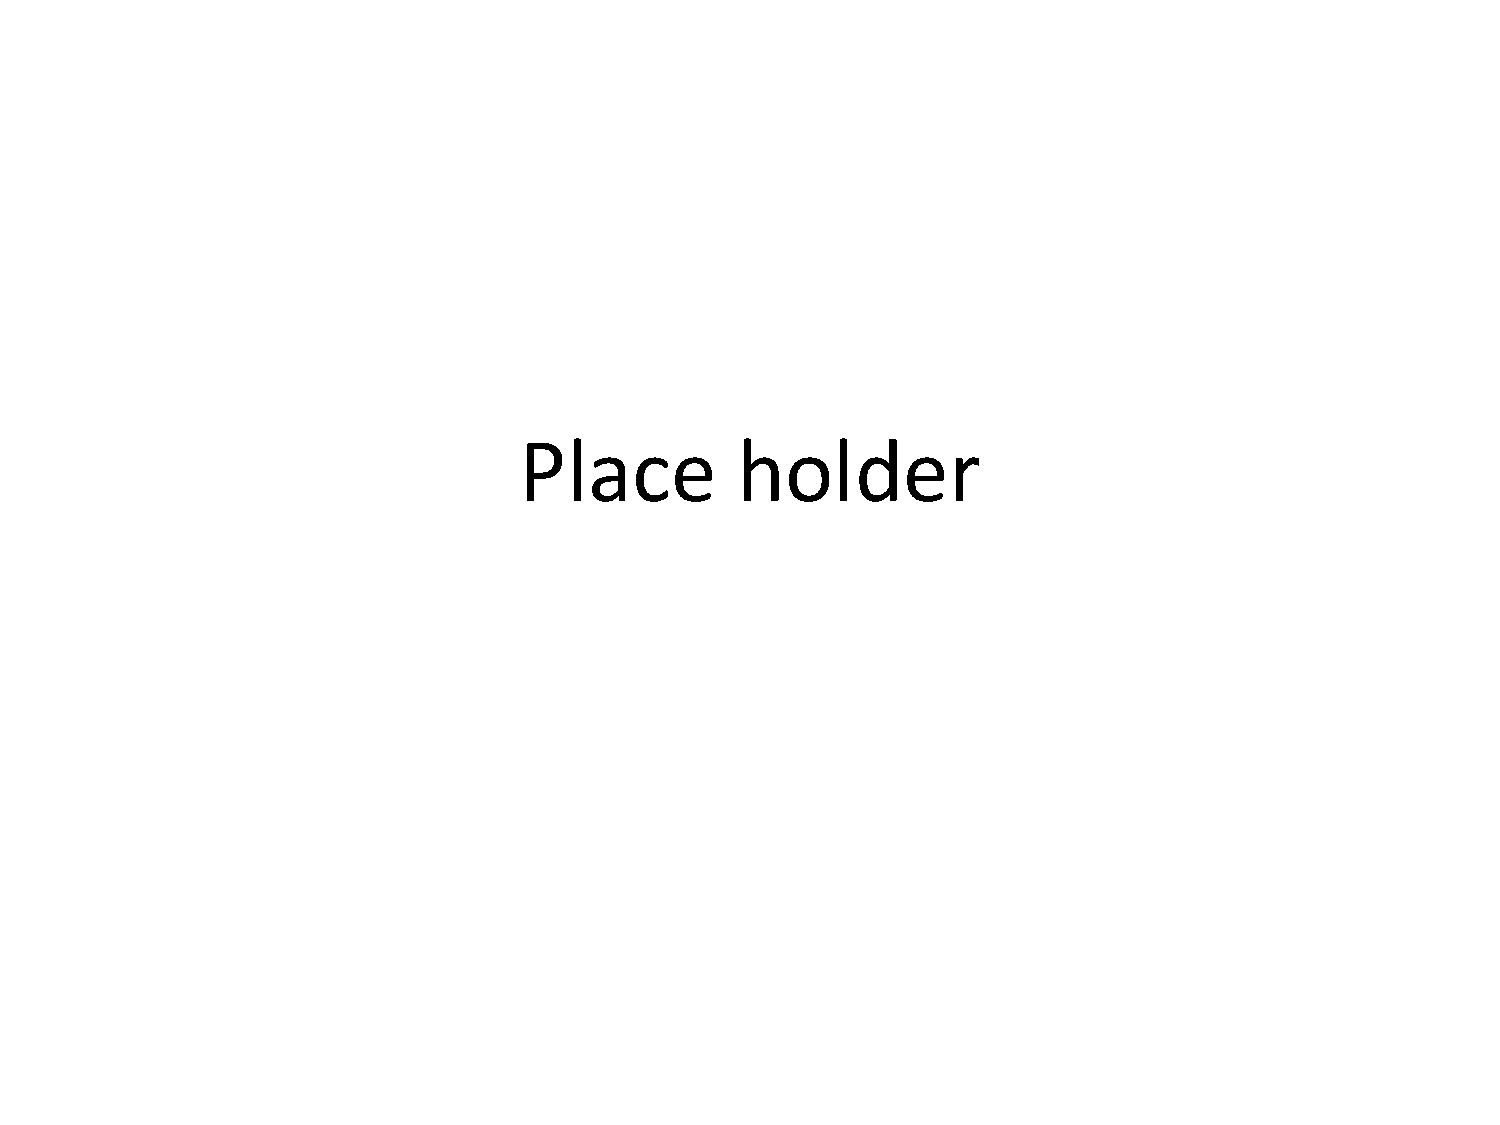
\includegraphics[scale=0.2]{placeHolder.pdf}
	\caption{Open loop testing setup: the device (pacemaker) is fed with pre-programmed open-loop tests.}
	\label{fig:OLtestingSetup}
\end{figure}
Today, pacemakers are tested in an open loop \todo[inline]{cite}.
That is, the pacemaker is not connected to the heart, as shown in Fig.\ref{fig:OLtestingSetup}.
Rather, the validation engineer provides the DUT with $N$ open-loop tests
\[A_{OL} = \{\yb_k, k=1,\ldots,N\}\]
E.g., each test is a string of $A_{sense}$ and $V_{sense}$ values. The validator observes the DUT's output $\ub$ to determine correctness.
The tests $\yb_k$ are meant to mimic some possible signals produced by the heart and are designed in consultation with physicians.
They are also \emph{the same tests that were used when designing the pacemaker}.
\todo[inline]{check that last statement}
What the pacemaker's reaction should be is decided based on a diagnosis of the heart signals $\yb_k$:
that is, the physician diagnoses what might cause the heart to produce a certain $\yb$, and decides accordingly what the pacemaker should do.
The heart is thus only implicitly involved in the testing process. 
How does this compare with the ideal state of affairs outlined in Section \ref{testingObjectives}?
\begin{itemize}
	\item Choice of inputs:	There is no guarantee that the validator's tests satisfy $A_{OL} = A_
	Hc$. 
	Thus testing might miss valid test cases ($\yb \in A_\Hc \setminus A_{OL}$), or include irrelevant ones ($\yb \in A_{OL} \setminus A_\Hc$).
	Moreover, there is no automatic way of producing the tests: rather, it is a manual and error-prone process.
	\item Criterion of correctness: because the heart does not figure in open-loop testing, correctness is decided based on the pacemaker's reactions. 
	What these mean for the heart is only implicit or assumed, but is not actually tested. 
	While there is no substitute for the physician's expertise, the fact that they need to diagnose every test means there will be inevitable errors or lapses.
\end{itemize}

In the next section, we present a closed-loop testing setup which addresses both shortcomings of open-loop testing.

\subsection{Closed-loop testing of pacemaker}
\label{closedloop}

\begin{figure}[t]
\centering
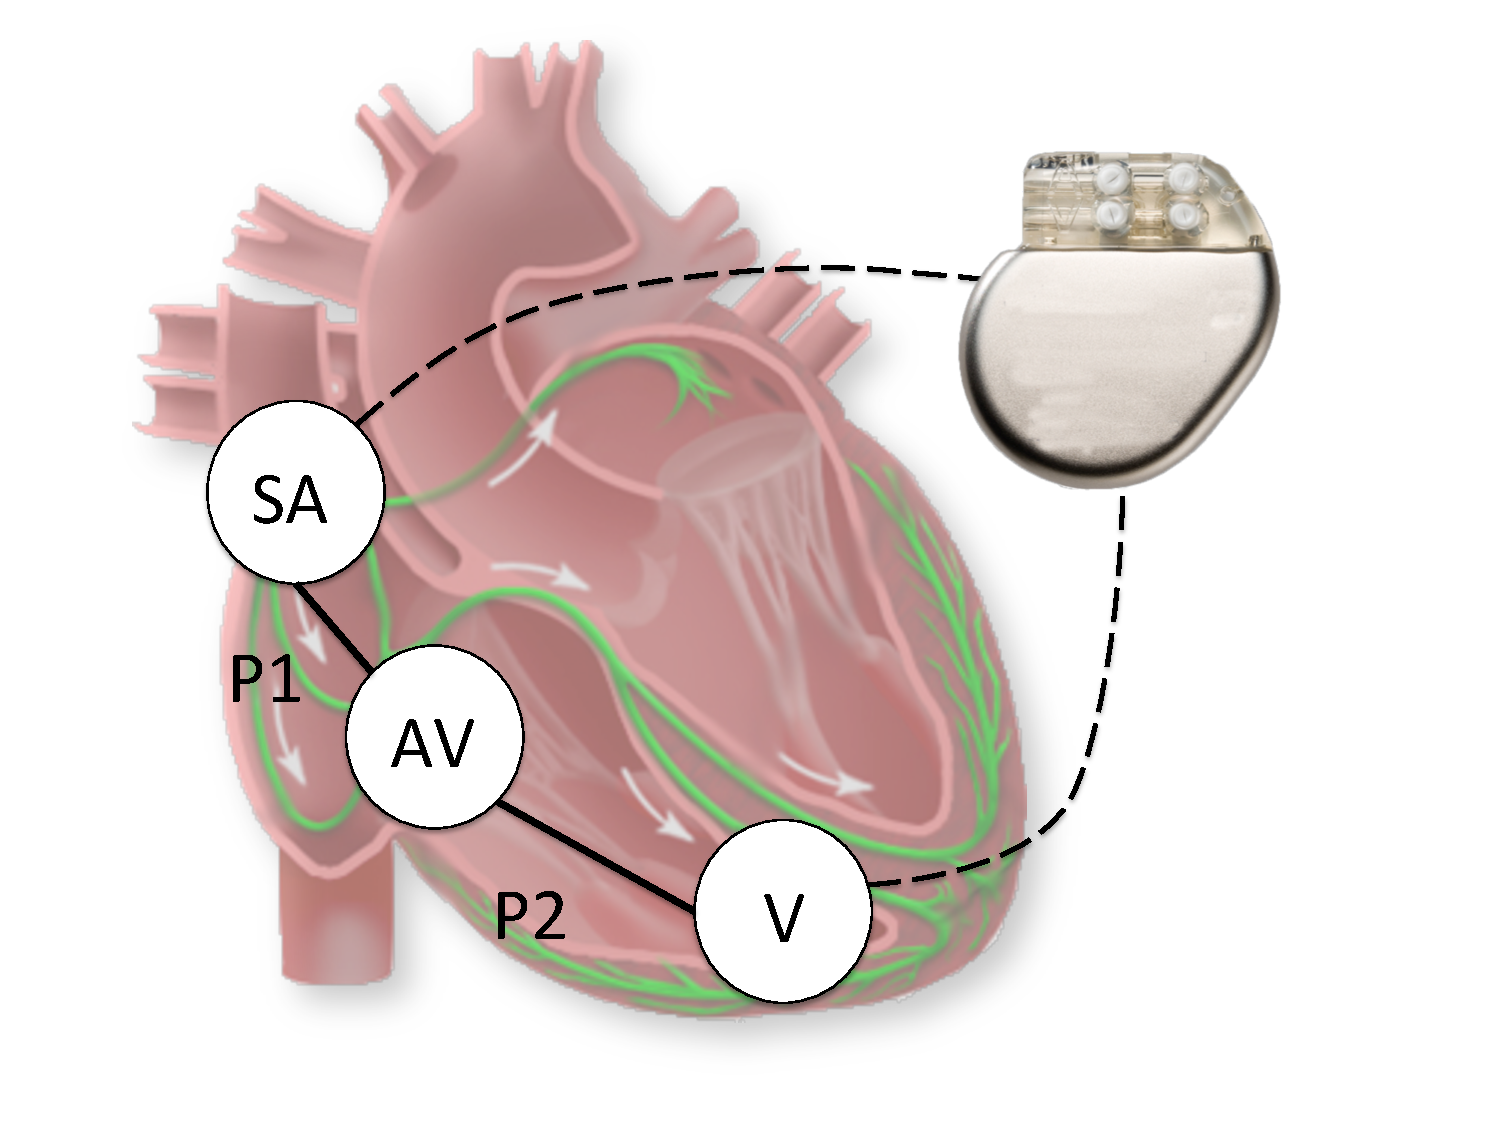
\includegraphics[scale=0.2]{figures/nodesandPM}
\caption{Portion of the VHM: the conduction paths P1 and P2 connect the SA node to the ventricle via the AV node (solid line). The pacemaker induces a second, `virtual', pathway (dashed line).}
\label{fig:nodesandPM}
\end{figure}

\textbf{Closed-loop setup}.
The closed-loop setup is shown in Fig.~\ref{fig:reqGuidedTesting}.
The VHM and pacemaker are connected in the same way as a real heart and pacemaker would be connected.
Thus, the inputs to the pacemaker are automatically generated by the VHM as atrial and ventricular sensing events (AS and VS, respectively), and don't need to be pre-programmed by the validation engineer. 
The VHM, in turn, is stimulated by the pacemaker's Atrial and Ventricular Pacing events (AP and VP).
In addition, the tester is connected at the PVC `inputs' to the heart.
That is, the tester provides waveforms that mimic Premature Ventricular Complex (PVC) events in the ventricle.
Thus, PVCs also don't need to be pre-programmed by the validation engineer.
The tester can read all required signals from the VHM and pacemaker model.
In our experiments, it reads five waveforms from the closed loop: the depolarization events at SA node, AV node, and ventricle (SA, NA and V), and the conduction state of paths P1 and P2 connecting them. (See Fig.~\ref{fig:nodesandPM}.)
It also reads the AP and VP events from the pacemaker.

\textbf{Tester-controlled inputs}.
In our setup, the testing algorithm will generate PVC waveforms to mimic the abnormal depolarizations of the ventricles that occur in a heart with arrhythmia. 
A \emph{test} is then defined as a PVC waveform of a pre-determined duration $T$ ms.
These are used by the tester to try and cause the closed loop to manifest unsafe or undesirable heart conditions.
The constraint on the waveforms generated by the tester is that there should be at least 400ms between consecutive PVC impulses.

\textbf{The tester}.
The tester itself is a specification-guided automatic test generation algorithm, whose theory can be reviewed in \cite{AbbasFSIG13tecs}, and we review it here briefly.
This testing algorithm has been implemented in the tool S-Taliro \cite{AnnapureddyLFS11tacas}, and has been used in other medical applications like the analysis of insulin infusion pumps schedules \cite{SankaranarayananF2012cmsb}.
The operation of the tester is as follows: we provide S-Taliro with a specification that the pacemaker+heart closed loop must satisfy,
e.g., ``there should be a minimum delay of 500ms between VP events''.
S-Taliro then generates a sequence of tests, i.e., a sequence of PVC waveforms, each of a pre-determined duration $T$ ms.
After each test, S-Taliro observes the outputs from the system and calculates \emph{the degree} to which the specification is satisfied or not.
This degree is then used to choose the next test to apply. 
It can be shown that if the system can exhibit a behavior that violates the specification, then this iterative process converges to a test that will provoke this incorrect behavior \cite{AbbasF_HybridSA12}. 
This test then serves as evidence that the pacemaker+heart loop can exhibit undesired behavior that violates the specification.
The pacemaker's designer can then replay this test to see where things went wrong, and whether the pacemaker needs to be adjusted accordingly.

\textbf{Advantages over open-loop testing}.
The advantages of the proposed specification-guided closed-loop testing approach over directed open-loop testing are summarized in Table \ref{table:CLoverOL}, and discussed here:
\begin{table*}
	\centering
	\caption{Comparison between open-loop and proposed closed-loop testing.}
	\begin{tabular}{|l|l|l|}
	\hline                       & Open-Loop    & Requirements-Guided Closed-Loop 
	\\ 
	\hline Choice of pacemaker input traces  
	                & Manual and recorded traces. Might miss interesting behavior, &  Automatic and provided by the VHM,
	\\ 
					& or include irrelevant behavior. &  so only relevant input traces are used.
	\\
	\hline Criterion of correctness    & Only pacemaker behavior & The heart and pacemakers's joint behavior, so 
	\\
	                &                  & physiological effects of pacemaker actions
	\\
	                &                  &  can be used to determine correctness.                   
	\\ 
	\hline Choice of tests & Tests = input traces to pacemaker.  & Tests = traces of external disturbances, 
	\\
	                & Manually chosen.  & like PVC and PAC. Automatically selected by S-Taliro.
	\\
	\hline 
\end{tabular}
\label{table:CLoverOL}
\end{table*}

\begin{figure}[t]
\centering
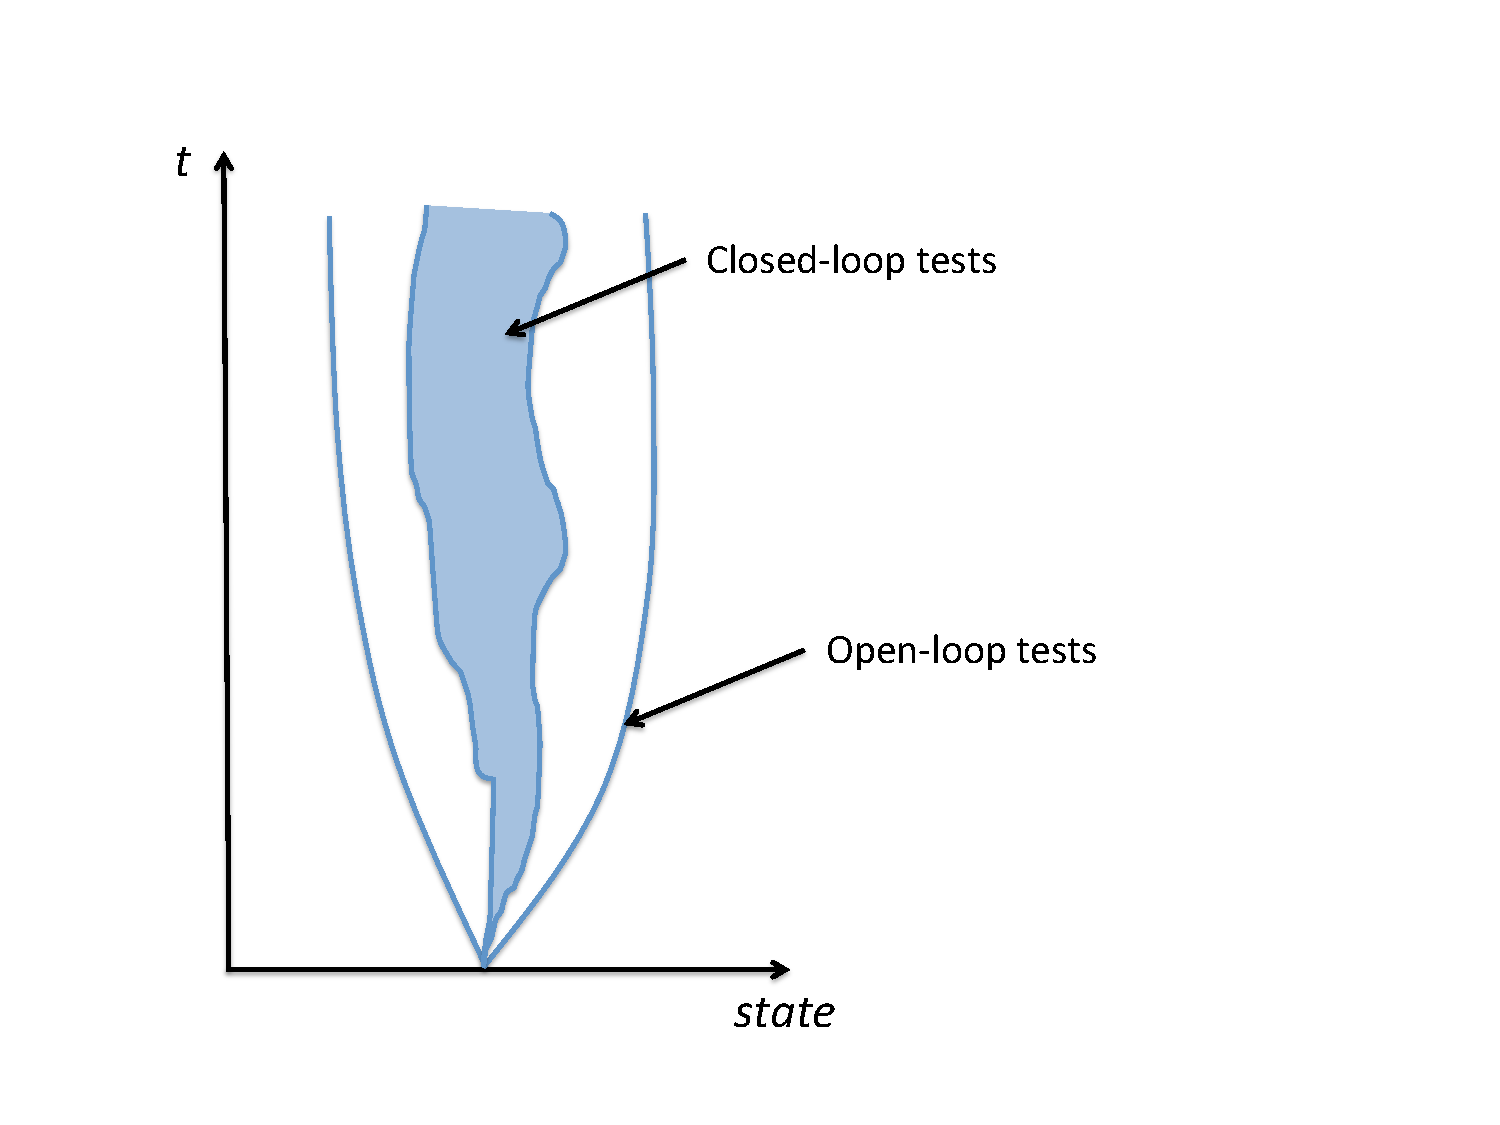
\includegraphics[scale=0.4]{figures/cone}
\caption{The space of closed-loop inputs to the pacemaker is constrained by the VHM and is thus smaller than the open-loop space.}
\label{fig:cone}
\end{figure}

\begin{itemize}
	\item Choice of inputs: because a heart model provides the input traces to the pacemaker, we know that only relevant test cases will be generated and fed to the pacemaker. 
	That is, only traces that the pacemaker may actually see during live operation are fed to it during testing. 
	\footnote{Of course, this ultimately depends on the quality of the VHM.}
	Compare this to open-loop testing where theoretically, the space of open-loop tests is much larger since nothing constrains the inputs, as illustrated in Fig.~\ref{fig:cone}.
	It is difficult if not impossible to reason a priori about how the heart will constrain the pacemaker's inputs, especially for \emph{deep} behaviors that take a long time to occur.	
	Moreover, because the tester produces the tests systematically, we are guaranteed to find violating behavior if it exists.
	\item Criterion of correctness: because we have a VHM, we can express correctness \emph{as a property of the heart's behavior}, and not of the pacemaker alone. 
	Thus we can evaluate what truly matters: is the heart (as modeled by the VHM) displaying unsafe or undesirable behavior?
\end{itemize}

%\textbf{Choice of specifications to test}.
%Because the heart's behavior is complex and varies depending on its physiological structure and history, it is not always easy to describe succinctly what is `unsafe' and what is `undesirable'.
%Both categories vary depending on what we know (and what we discover) about the heart conditions being modeled.

\textbf{Interpretation of testing results}.
It must be stressed that the interpretation of closed-loop testing results depends on the specific violating behaviors that are found.
Some will be determined to be bugs in the pacemaker (or VHM). 
Others will be determined to be undesirable but necessary behaviors, and we show such a case in Section \ref{experiments}.
This is because specifying `safe' behavior can be difficult for something as complex as the heart.

\section{Experiments}
\label{experiments}

%a) \emph{Debugging the pacemaker}: As an illustration of how a Virtual Heart Model (VHM) can be used to debug a pacemaker, we give a simple example of a pacemaker model in Simulink, connected to a VHM in Simulink as well. 
%No open-loop testing was conducted on this pacemaker model.
%The requirement given to the tester was that if a PVC or VS or VP occur, then the next VP should not occur before 500ms. 
%\todo[inline]{ZJ : why is this a requirement of good behavior?}
%The specification-guided testing methodology outlined in Section \ref{closedloop} quickly found a PVC disturbance waveform that caused the closed loop to violate this specification (fewer than 10 tests).
%Debugging revealed that the pacemaker model was missing the behavior that caused it to reset the Upper Rate Interval to its default value after every VS event.

For the following two experiments, the pacemaker model is evaluated against two physiological requirements.

a) \emph{Exploring behavior}: In this experiment, we set a minimum delay of 400ms between PVC pulses, and tried to falsify the following specification:
``The interval between an activation of the ventricle node to a ventricular pacing (VP) should be longer than 500ms".
This specification is designed to identify closed-loop execution traces in which the pacemaker is pacing the heart too fast. %Note that the pacemaker can not distinguish between a VS caused by a PVC and a VS caused by path conduction.
%Thus we need access to the heart model to test this specification, and this can only happen in a closed-loop setting.

The specification was violated by the execution shown in Fig. \ref{fig:bug8_kept1}.
% This comes from bug8_kept1
\begin{figure}[tb]
\centering
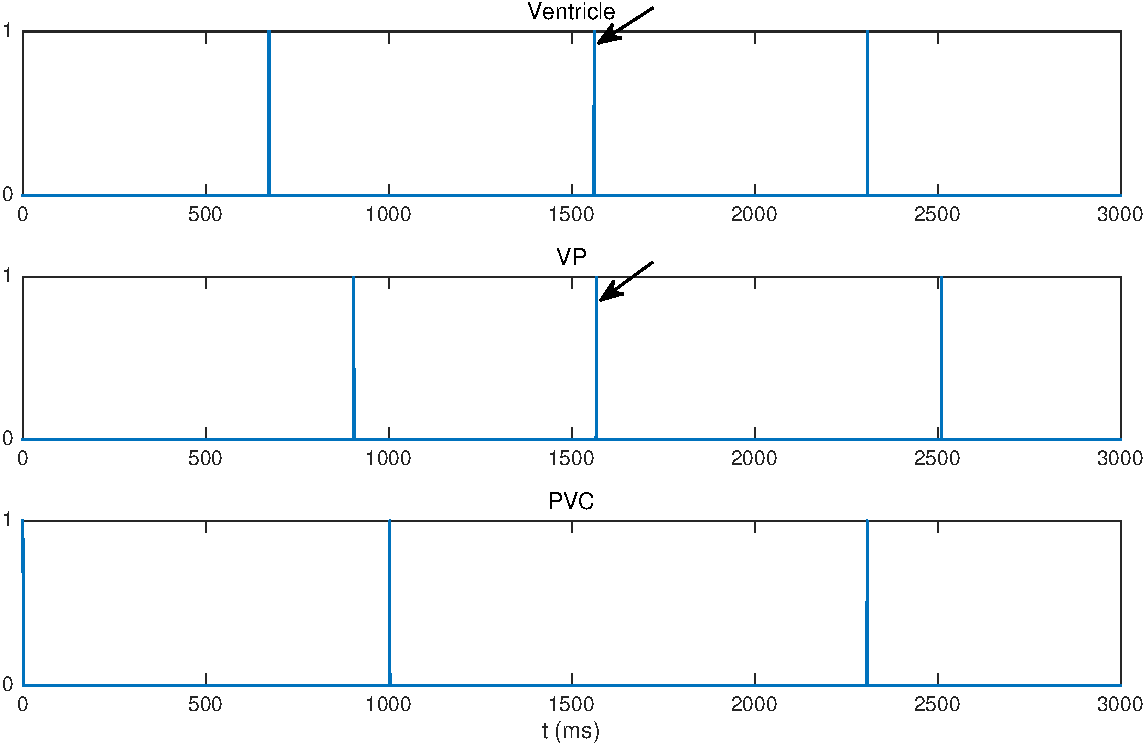
\includegraphics[width=0.7\linewidth]{figures/bug8_kept1}
\caption{A PVC pattern that causes a premature ventricular pacing.}
\label{fig:bug8_kept1}
\end{figure}
Upon investigating the reasons for this violation, it was concluded that one of the noise filter post-atrial ventricular blocking (PAVB) designed to avoid crosstalk between channels caused the problem.  
A PVC happened shortly after an atrial sense (AS) which fell into the PAVB period and was ignored. 
Due to its limited sensing capability the pacemaker cannot distinguish noise from a valid input which happened at a rare time.
Thus, the designer and physician must decide whether this is an acceptable case, or the pacemaker needs to be adjusted (if at all possible) to prevent this from happening (while maintaining the VSP safety feature).

b) \emph{Finding harmful heart behavior}: In this experiment, we tested the closed loop to see if the pacemaker could lead the heart into a harmful condition known as Endless Loop Tachycardia (ELT).
%
The heart has one intrinsic conduction pathway from atria to ventricles, namely from the SA node to the ventricles via the AV node and His bundle.
The AVI period of the DDD pacemaker introduces another, virtual, pathway between the atrial lead and the ventricular lead.
See Fig.~\ref{fig:nodesandPM}.
If a PVC happens shortly after a normal A-to-V conduction, the signal would go around the closed circuit formed by the heart and the pacemaker, inhibiting intrinsic heart signals and causing the heart to beat at a fixed high rate.
First, the PVC triggers V-A conduction along the intrinsic pathway, 
which in turn triggers Atrial Sense (AS). 
The pacemaker will then pace the ventricle (issue a VP) after TAVI ms according to its A-V synchrony function. 
This VP then triggers another V-A conduction, and so on.
The conduction loop is then formed and the VP-AS pattern will persist if no actions are taken.
The heart rate is kept as high as the upper rate limit of the pacemaker since the cycle length of the conduction loop is very short. 
ELT is a harmful condition since a fast fixed heart rate that will cause inefficient pumping of blood.
Thus even though the pacemaker is correct according to its specification, it can still lead the heart into ELT if a PVC interferes with its operation as described.
%

S-Taliro was given the ELT specification, and a PVC constraint of at most 2 PVCs in a 10,000ms interval. 
The total test duration was $T= 10,000$ms.
S-Taliro found a PVC pattern, shown in Fig.~\ref{fig:bug13_kept1}, that caused ELT.
% This is bug13_kept1
\begin{figure}[t]
\centering
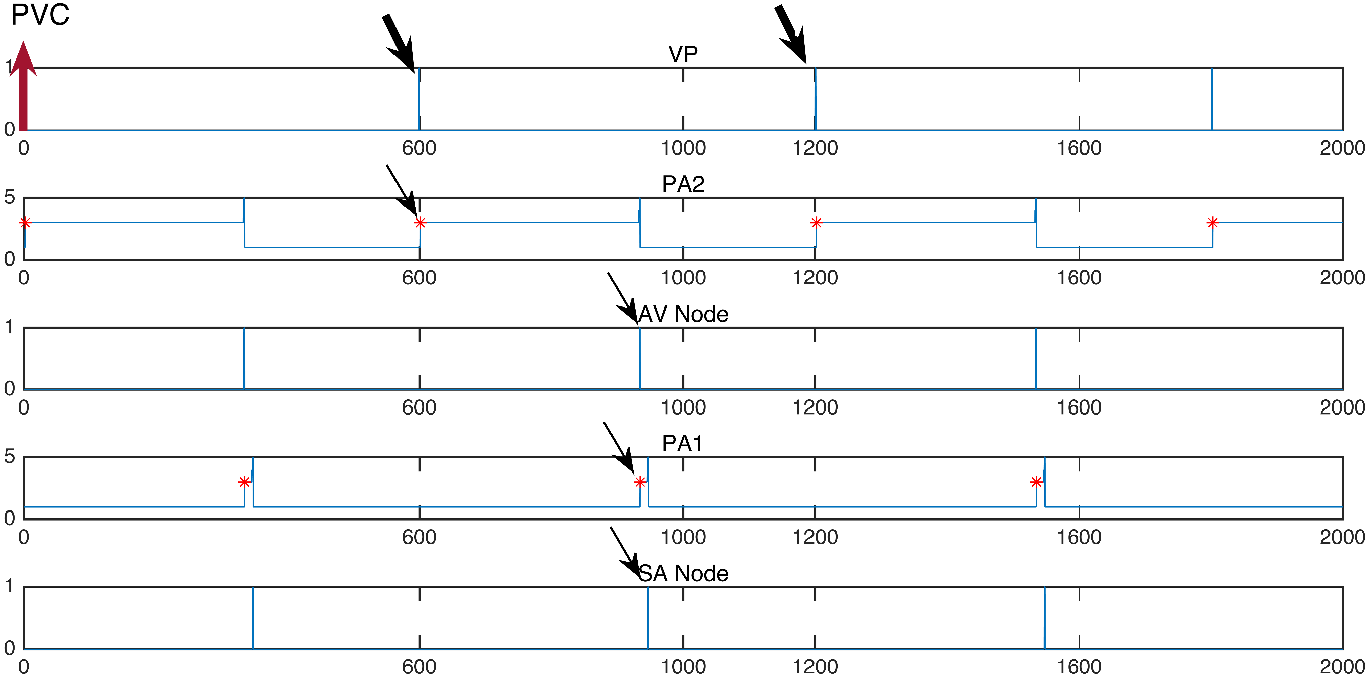
\includegraphics[height=0.2\textheight,width=1\columnwidth]{figures/markedELT.pdf}
\caption{ELT. The vertical red arrow indicates the initial PVC, thick arrows indicate the beginning of each ELT cycle, and thin arrows indicate the events involved in the ELT diagnosis.}
\label{fig:bug13_kept1}
\end{figure}








\end{document}
